\documentclass{article}
\usepackage[utf8]{inputenc}
\usepackage{graphicx}

\title{TPL POO : Robots}
\author{Salah-Eddine Bariol Alaoui\\Majd Fariat\\Dimitri Pierucci}
\date{November 2016}

\begin{document}

\maketitle

\section{Première partie : les données du problème}

\subsection{Implémentation des Robots} \\

Comme demandé dans le sujet, la classe robot est abstraite, et possède une architecture particulière, cette architecture est détaillée dans la figure suivante: \\

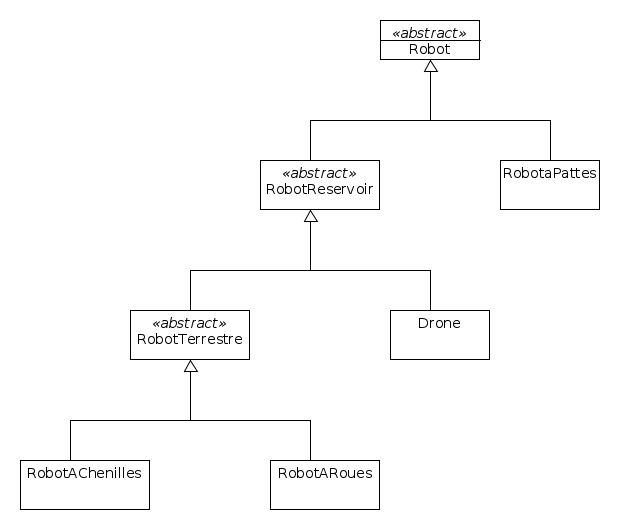
\includegraphics[scale=0.5]{UML-Robot.jpg} 

\noindent Nous avons tout d'abord décidé de séparer les robots qui fonctionnait avec un réservoir à eau et le robot à pattes qui lui fonctionne avec de la poudre et qui possède un reservoir considéré comme infini. Cette séparation nous permet de factoriser plusieurs méthodes liées à la gestion de l'eau du robot. La classe \textbf{RobotReservoir} est abstraite : elle permet simplement d'éviter la redondance de code. \\
Ensuite nous avons séparé \textbf{RobotReservoir} en deux classes: la classe drone, qui implémente donc un drone et qui est donc finale, et une autre classe abstraite \textbf{RobotTerrestre} qui permet de factoriserle code qui gère le remplissage des robots (les tobots à roues et à chenilles se remplissent de la même manière). Enfin les classes \textbf{RobotsAChenilles} et \textbf{RobotARoues} implémentent la classe \textbf{RobotTerrestre}, et sont bien sur finales. 

\subsection{Implémentation de l'interface graphique} 

La classe \textbf{Simulateur} implémente l'interface graphique, comme expliqué dans l'énoncé, cette dernière implémente l'interface \textbf{Simulable}. Les principaux attributs de cette classe sont la GUI \textbf{gui}, les données de la simulation \textbf{donnees} (carte, robots, incendies) ainsi que la liste d'evnement que nous détaillerons dans les parties ultérieures. Cette classe affiche la carte et la met à jour à chaque évenement.

\section{Deuxième Partie : simulation de scénario}

\subsection{Gestionnaire d'évènements discret}

Ici peu de libertés ont été prises par rapport à l'énoncé : la date courante est représenté par un entier et incrémentée de 1 à chaque "pas" temporel. Le fonctionnement est très proche de ce qui est détaillé en annexe. 

\subsection{Evenements} 

Tout comme pour les robots la classe Evenement est abstraite, nous avons implémenté trois types d'évenements 
\begin{itemize}
    \item \textbf{EvenementDeplacementRobot} : a pour attribut supplémentaire une direction, il déplace le robot dans la direction donnée.  
    \item \textbf{EvenementDeverserEau} : a pour attribut spécifique l'incendie sur lequel deverser l'eau et l'index de l'incendie dans la liste des incendies, il indique au robot qu'il doit deverser de l'eau sur un incendie, si le robot a assez d'eau pour éteindre l'incendie, il ne met que la quantité d'eau correspondant à l'intensité de l'incendie. SI le robot n'a pas assez d'eau, il vide complétement son réservoir, mais l'incendie ne sera pas complétement éteint.
    \item \textbf{EvenementRemplir} : remplit le robot, si la case n'est pas valide (drone qui ne se situe pas sur une case d'eau par exemple), renvoit une exception. 
\end{itemize}

\section{Trosième Partie : calculs de plus court chemins}

\subsection{Structure de l'implémentation de la partie 3}

Le calcul du plus court chemin est délégué à la classe Chemin, qui a pour attributs une liste d'évenements qui correspondent aux déplacement élementaires (dans une des 4 directions) qui déterminent le chemin vers la destinantion voulue. La classe Chemin a aussi pour attribut une date, qui correspond à la date de début du chemin.

\subsection{Choix de l'algorithme}

Nous avons ici opté pour l'algorithme de Djikstra, permettant de calculer le plus court chemin vers la destination. 

\section{Dernière Partie : résolution du problème}

Nous avons opté pour la stratégie élémentaire. Il s'agit de parcourir dans 2 boucles imbriqués les incendies qui sont sur la carte, et de parcourir pour chaque incendie la liste des robots pour voir lequel est disponible


\end{document}
